\chapter{Assignment C: Global and Local Coordinate Systems}
The main objective of the assignment is to grasp the transformation from the global coordinate system (WGS84) to the local East-North-Up (ENU) coordinate system. With this relationship, satellite positions can be projected to the local ENU coordinate system. Furthermore, the visibility of a given satellite can be determined by checking its elevation angle.

\section{Theory}
According to~\cite{misra2006global}, the transformation from the WGS84 frame to the ENU frame can be computed as:
\begin{align}
\left[\begin{matrix}
x_{ENU} \\
y_{ENU} \\
z_{ENU} \\
\end{matrix}\right] &= \mathbf{R}_{WGS84}^{ENU}
\left[\begin{matrix}
x_{WGS84} \\
y_{WGS84} \\
z_{WGS84} \\
\end{matrix}\right] \\
\mathbf{R}_{WGS84}^{ENU} &= \mathbf{R_1}(90^{\circ}-\phi)\mathbf{R_3}(90^{\circ}+\lambda) \\
\mathbf{R_1}(\alpha) &= 
\left[\begin{matrix}
1 & 0 & 0 \\
0 & cos(\alpha) & sin(\alpha) \\
0 & -sin(\alpha) & cos(\alpha) \\
\end{matrix}\right]\\
\mathbf{R_3}(\alpha) &= 
\left[\begin{matrix}
cos(\alpha) & sin(\alpha) & 0 \\
-sin(\alpha) & cos(\alpha) & 0 \\
0 & 0 & 1 \\
\end{matrix}\right]
\end{align}
Once the coordinates in the ENU frame is obtained, the azimuth, elevation, and zenith angles can be computed as follows:
\begin{align}
tan(\alpha_{azimuth}) &= \frac{x_{ENU}}{y_{ENU}} \\
cos(\alpha_{zenith}) &= \frac{z_{ENU}}{\sqrt{x_{ENU}^2+y_{ENU}^2+z_{ENU}^2}} \\
\alpha_{elevation} &= 90^{\circ}-\alpha_{zenith}
\end{align}
\section{Tasks}
\begin{itemize}
    \item Implement a \textsc{Matlab} function for transforming a point in the WGS84 frame to the local ENU frame.
	\item Implement a \textsc{Matlab} function that computes the azimuth, elevation and zenith angle.
	\item Read satellite positions for a given time epoch from a SP3 file and then convert the satellite positions to the ENU coordinates. Determine elevation and azimuth in the local coordinate system for the vectors to all GPS satellites at the given time epoch. Finally, determine the distances from origo to the satellites visible.
\end{itemize}
\section{Code}
Complementary functions: \\
\textbf{WGS842ENU: convert coordinates from WGS84 to ENU}:
\lstinputlisting{../../assignment/utils/WGS842ENU.m}
\textbf{calcAzimuthZenithElevation: compute the azimuth, zenith, elevation angle for a given point}:
\lstinputlisting{../../assignment/utils/calcAzimuthZenithElevation.m}
\textbf{sp3fileParser: parsing sp3 file.}:
\lstinputlisting{../../assignment/ex3/sp3fileParser.m}
\textbf{Entry}:
\lstinputlisting{../../assignment/ex3/ex3_enu_conversion.m}
\section{Experiments}
\subsection{Single Epoch}
The result is shown in Fig~\ref{fig:ex31}.
\begin{figure}[h]
	\centering
	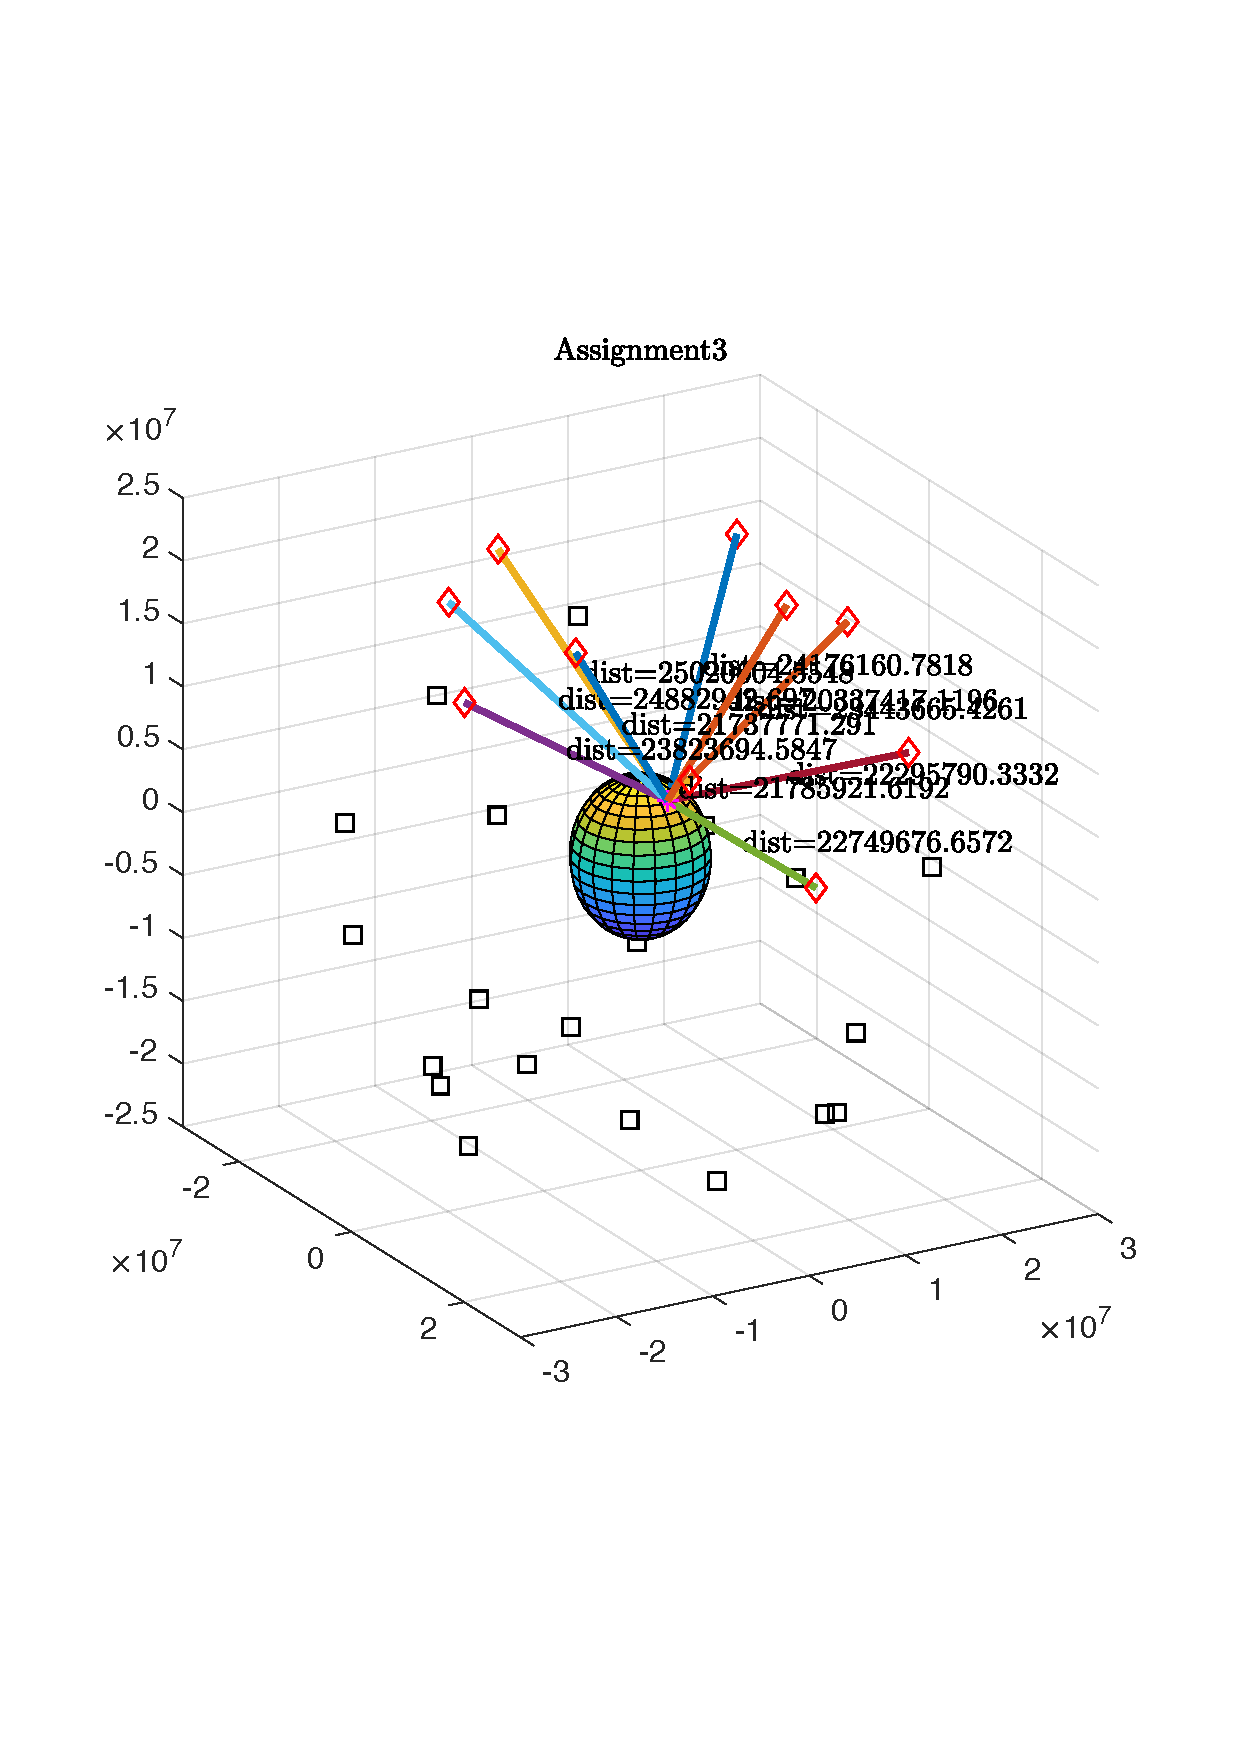
\includegraphics[width=\textwidth]{figures/ex31}
	\caption{Satellite visibili at a given epoch.}
	\label{fig:ex31}
\end{figure}
From the website of GPS.gov\footnote{\url{https://www.gps.gov/systems/gps/space/}}, it says that "GPS satellites fly in medium Earth orbit (MEO) at an altitude of approximately 20,200 km (12,550 miles)." Based on this data, it can be seen the calculated distances are reasonable since they are close to 20,200 km.

\subsection{Brute-force test}
In order to conveniently do more brute-force test, a \textsc{Matlab} GUI program is designed. The GUI program supports the following features:
\begin{enumerate}
	\item Automatically parse a sp3 file and list all relevant information.
	\item List all satellite positions' observations in a list box for the user to select.
	\item Input arbitrary latitude, longitude, and altitude.
	\item Visualization.
\end{enumerate}
Snapshots of the GUI program are shown as follows: \\
\textbf{Initialization}: \\
\begin{figure}[h]
	\centering
	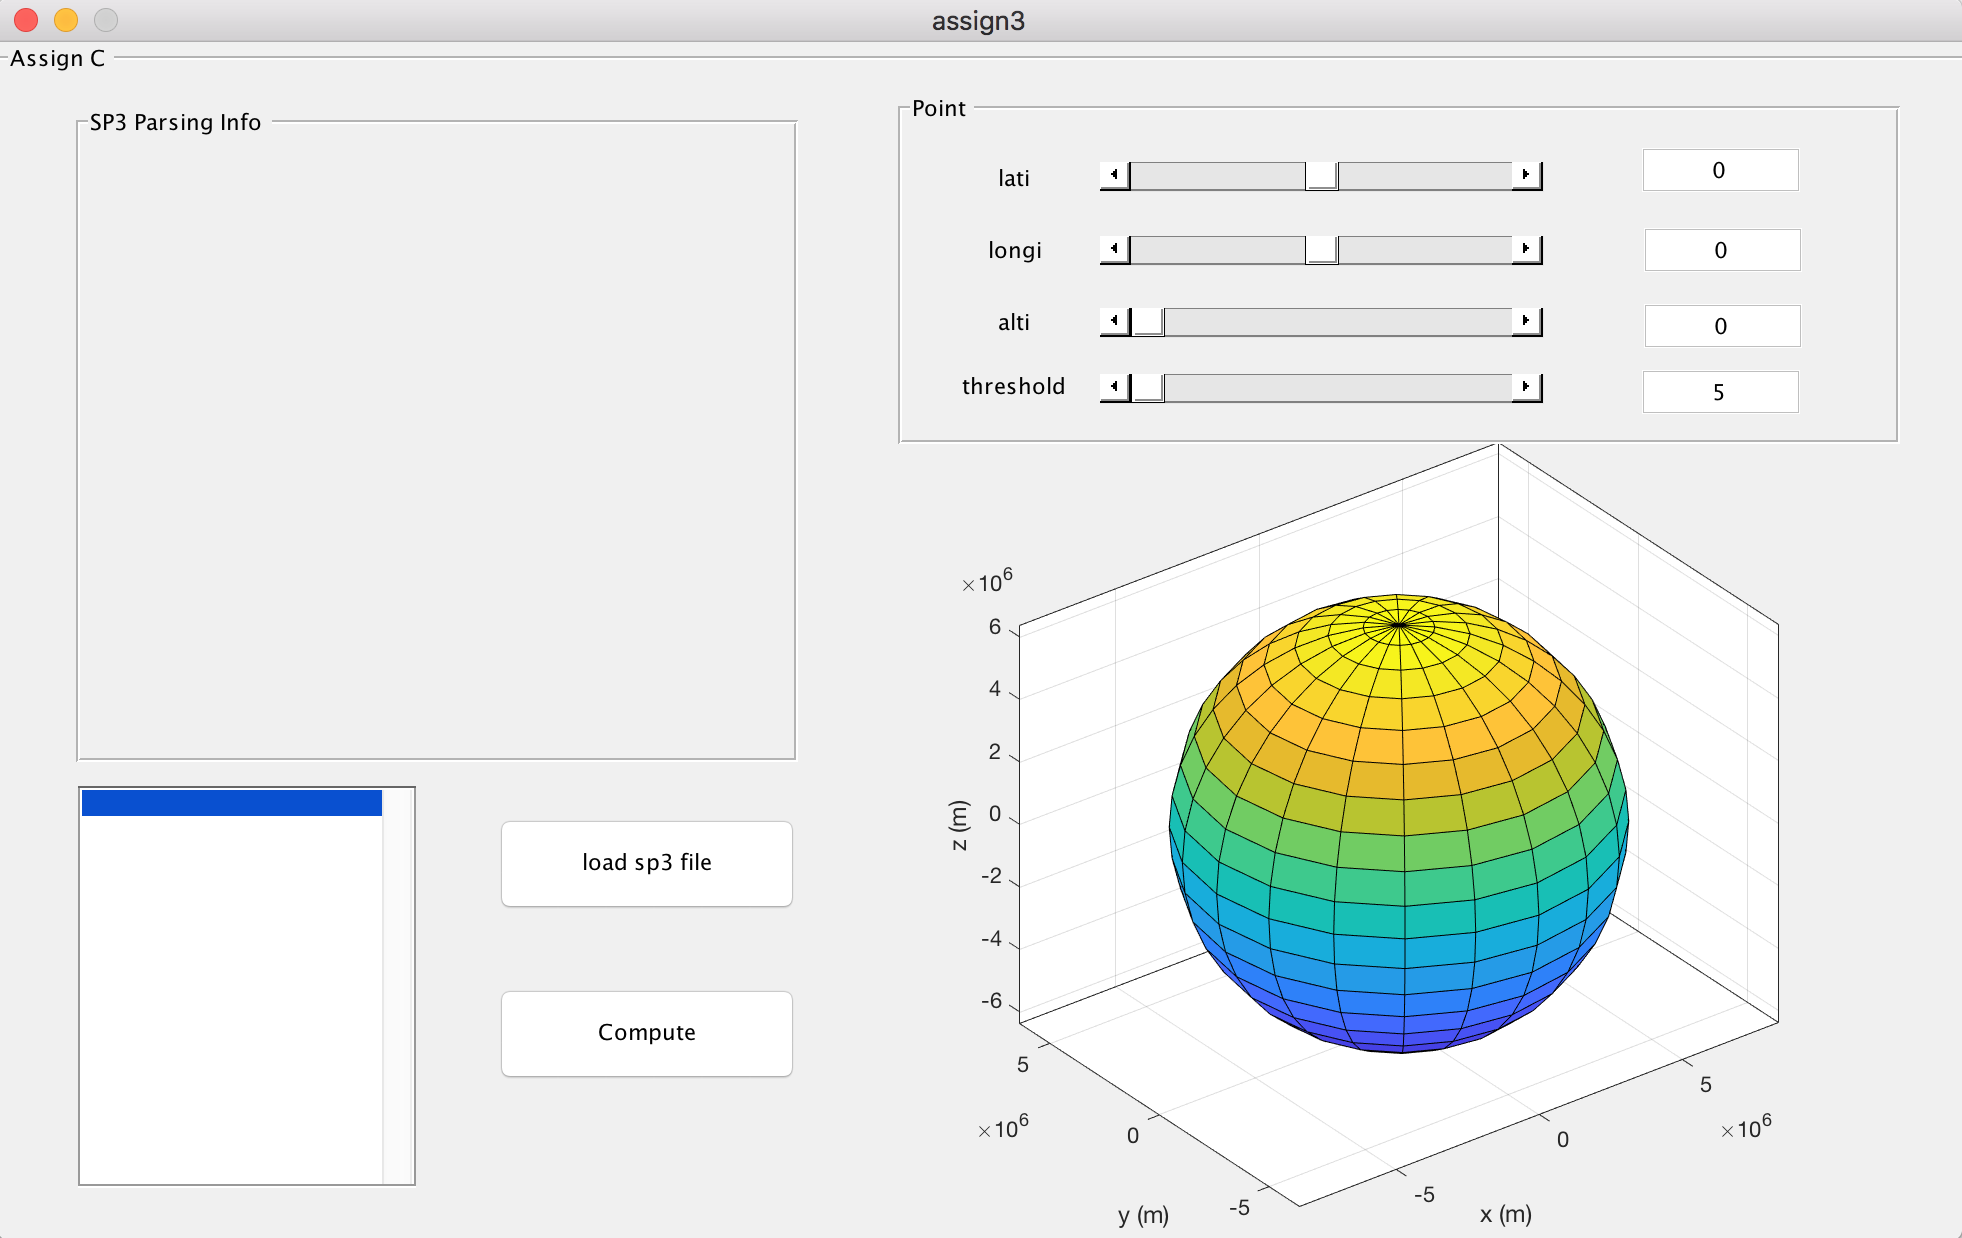
\includegraphics[width=\textwidth]{figures/ex3init}
	\caption{Initialization.}
\end{figure}
\textbf{After loading a sp3 file}: \\
\begin{figure}[h]
	\centering
	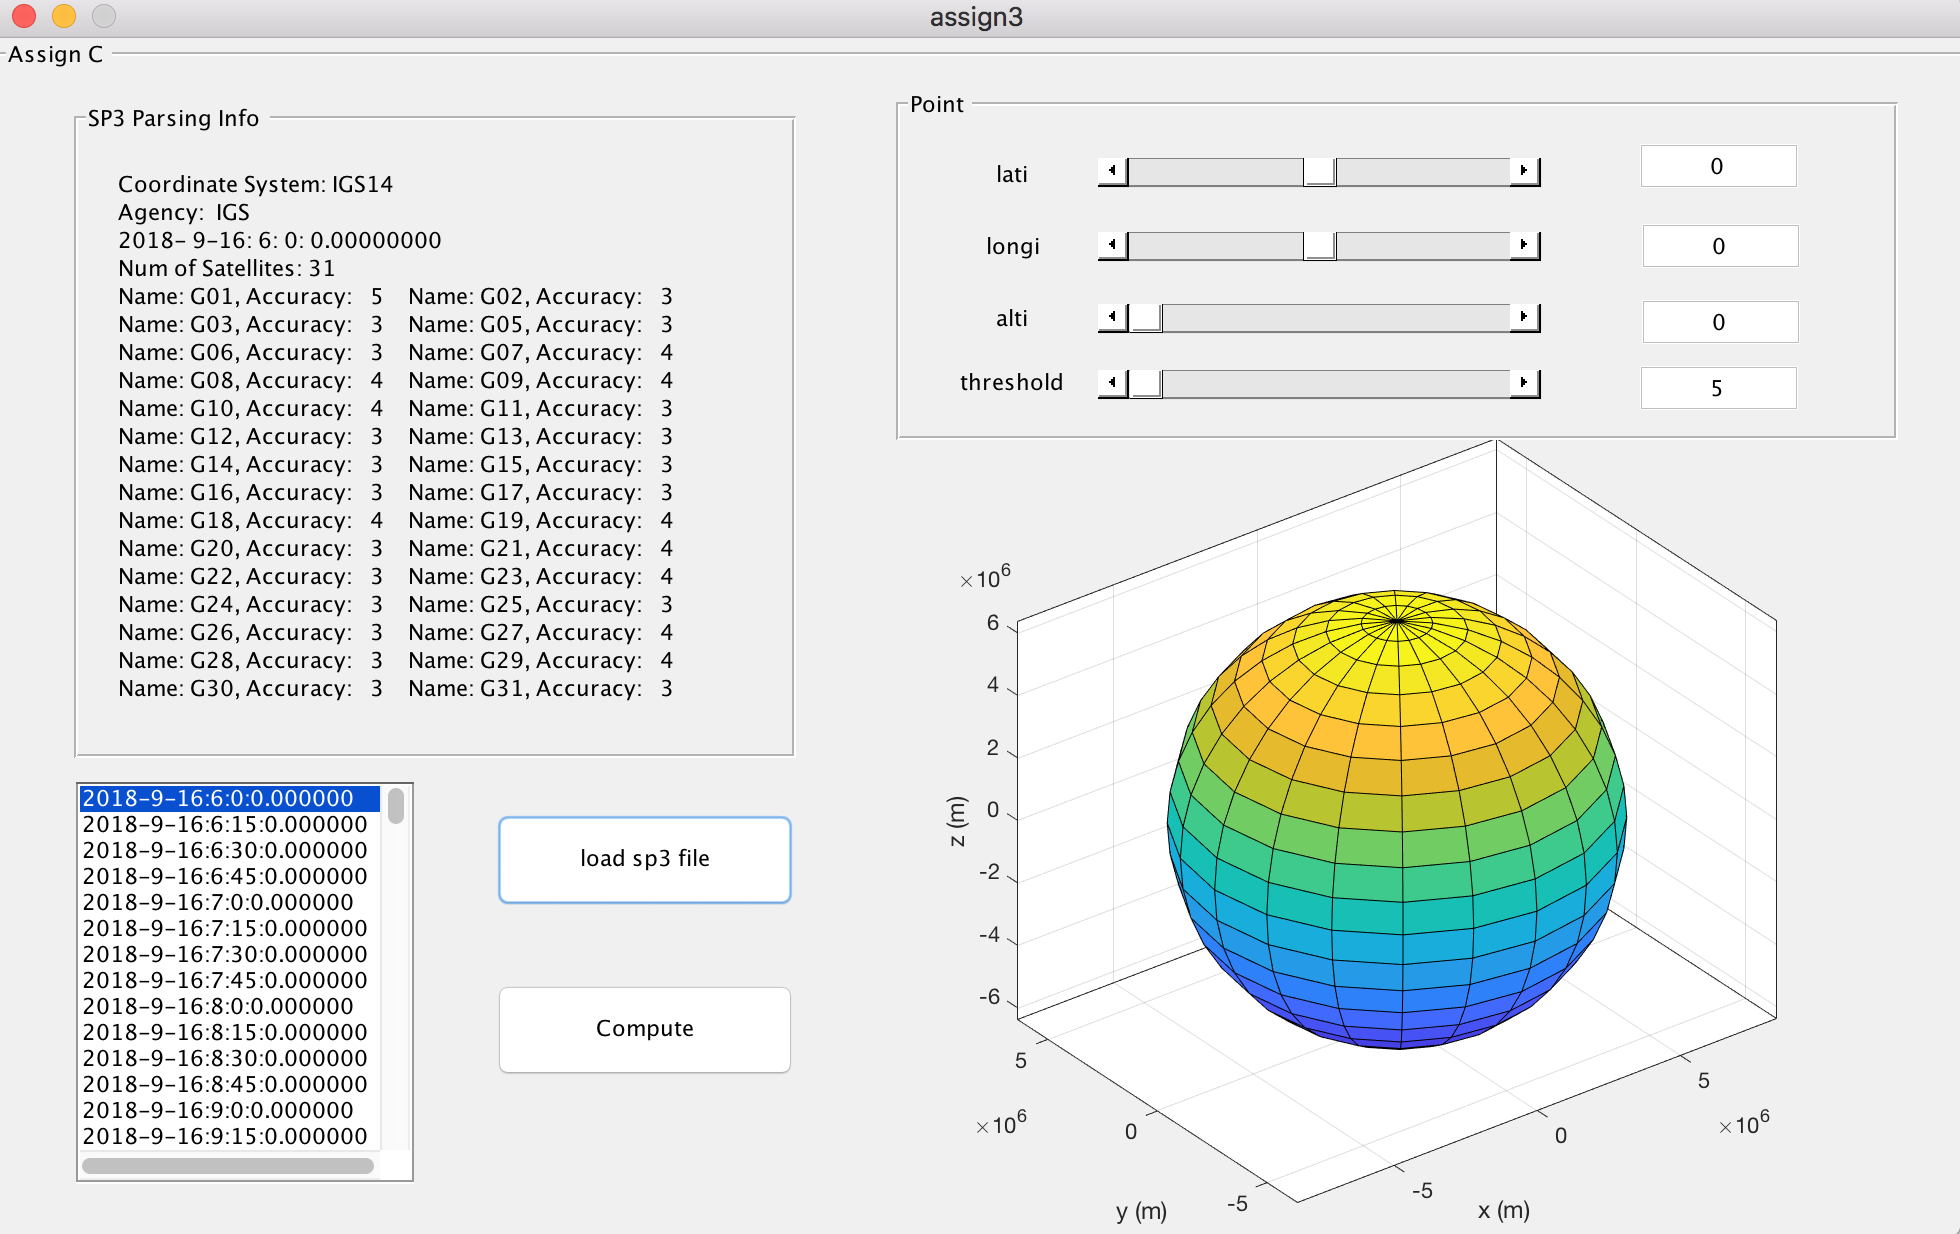
\includegraphics[width=\textwidth]{figures/ex3loadsp3}
	\caption{Loading a sp3 file.}
\end{figure}
\textbf{Results of 2 examples}: \\
\begin{figure}[h]
	\centering
	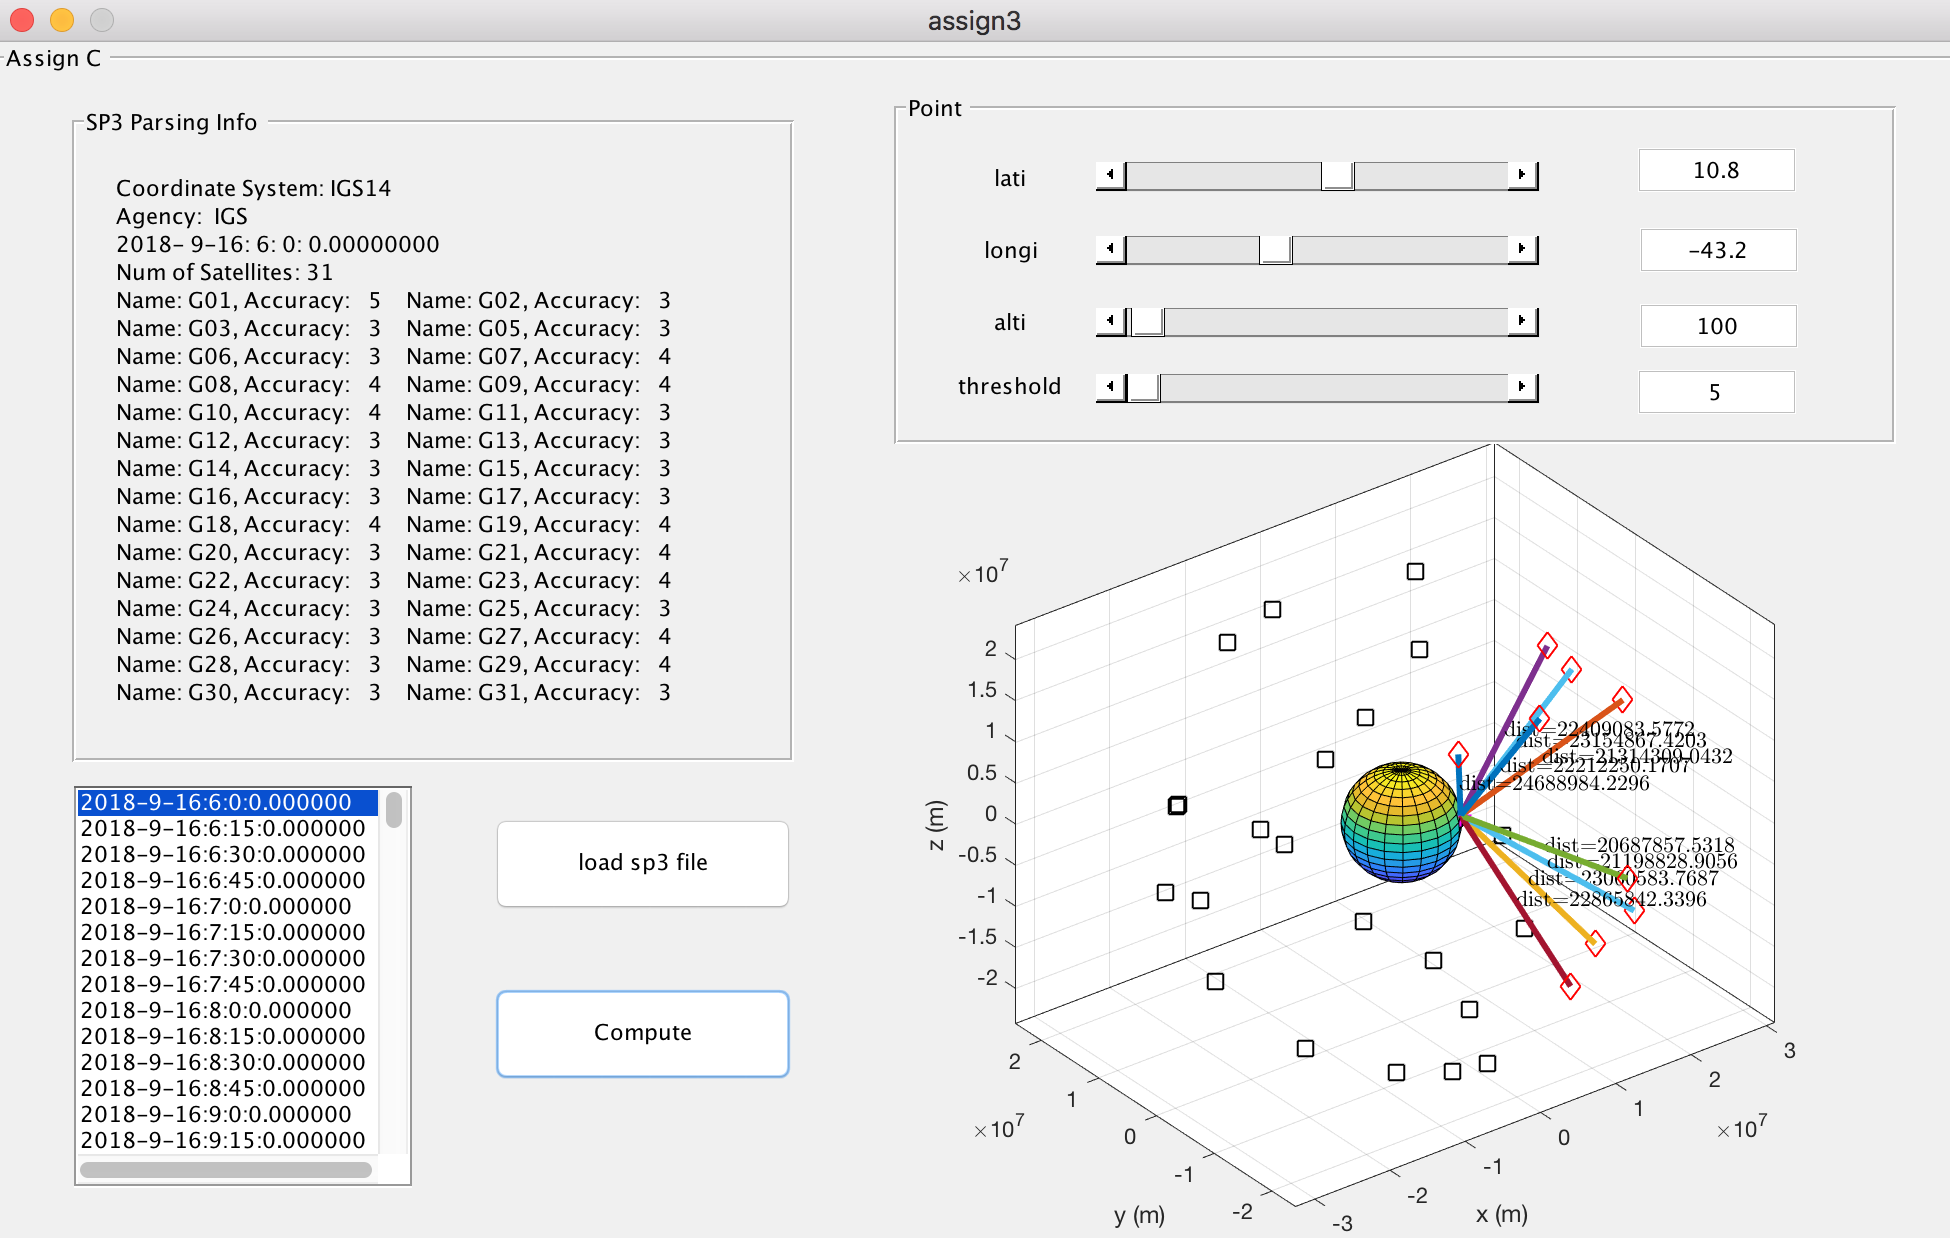
\includegraphics[width=\textwidth]{figures/ex3com1}
	\caption{Snapshot of the result 1.}
\end{figure}
\begin{figure}[h]
	\centering
	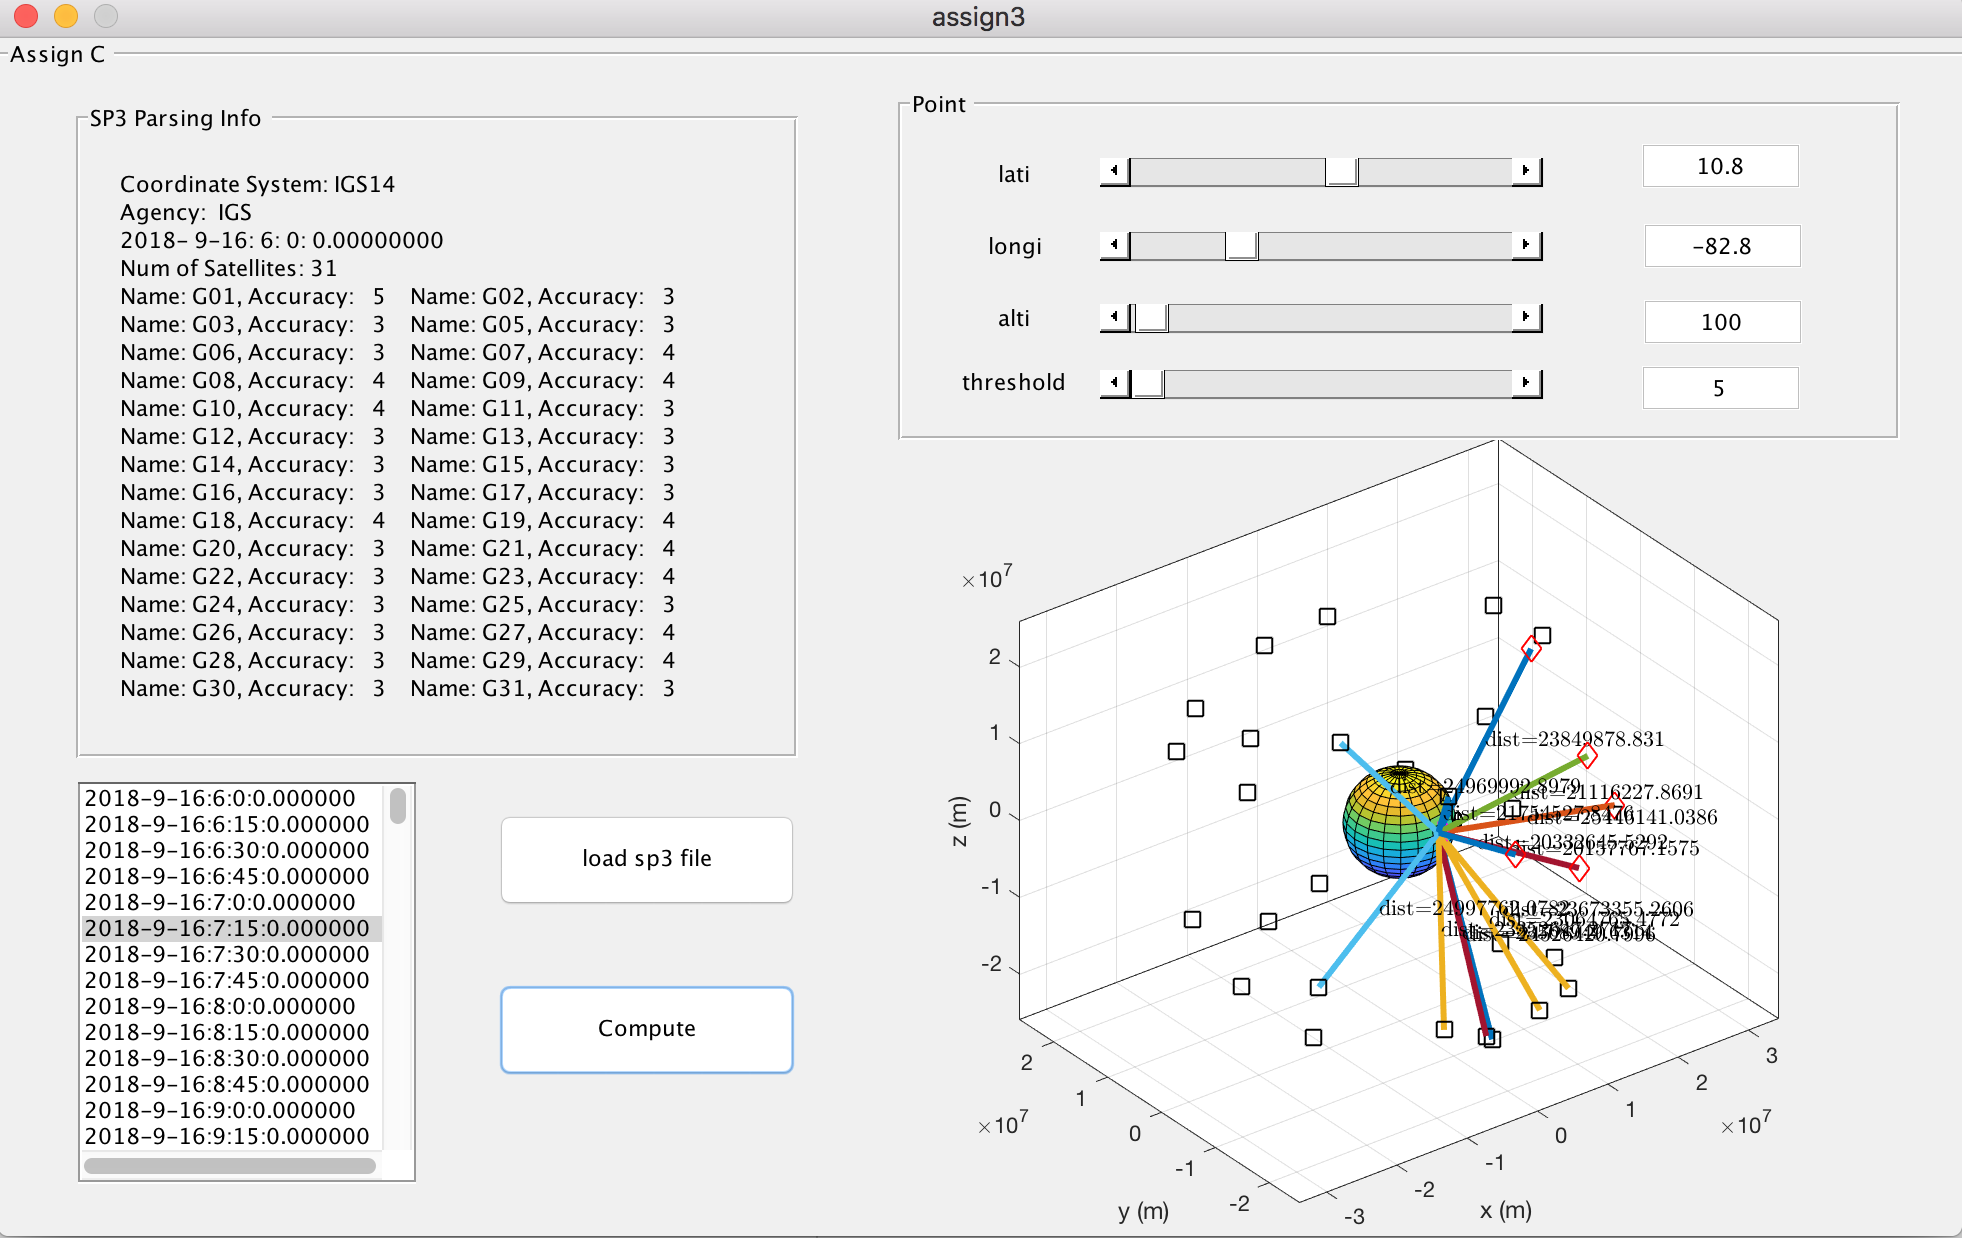
\includegraphics[width=\textwidth]{figures/ex3com2}
	\caption{Snapshot of the result 2.}
\end{figure}
\subsection{Conclusion}
Through this assignment, I grasp how to do the conversion from WGS84 to ENU frame and verify the visibility of a given satellite by checking its elevation angle. \\
I designed a GUI program that can easily parse a sp3 file, and do the conversion automatically. The program is easy-to-use.